\documentclass[../main.tex]{subfiles}
\graphicspath{{\subfix{../images/}}}

\begin{document}

\begin{newrequirements}
    \begin{todolist}
    \item Actual Design description with pictures 
        and diagrams. E.g., a “wiring diagram” 
        of the implemented hardware can be 
        added. 

    \item Actual images of various modules must 
        be included wherever possible. 
        Otherwise, at least the images of 
        various aspects of the completed design 
        must be shown. 

    \item List the different tools and framework 
        used for the implementation. 

    \item Discuss any novel aspects of your 
        implementation (if applicable). You may 
        link this aspect of your design to the 
        comparison table at the end of 
        literature review and elaborate on the 
        steps taken in achieving these 
        novelties in your design. 

    \item Discuss the challenges encountered 
        during the implementation and how they 
        were addressed. 

    \item You may organize any of the above 
        recommended points as subsections 

    \end{todolist}
\end{newrequirements}
In this section are going illustrate the actual design 
implementations, to achieve the design solution.
\subsection{Hardware}

The most critical parts in the hardware
architecture are the Raspberry Pi and the drone. 
We started by configuring the Raspberry Pi micro\textsc{sd} card,
flashed it with Ubuntu 20.04 desktop version,
and installed Parrot Olympe successfully in virtual environment. 
Then, we plugged in the Wi-Fi dongle adapter
in a \textsc{usb}~2.0 port in the Raspberry Pi, 
and the \textsc{os} discovered it automatically. 
There were some challenges in setting up the connection automatically 
once the Raspberry Pi boots up. We discovered that some packages were not installed properly,
so we reinstalled the whole system again, and the problems has been addressed. 


Regarding the power supply, we were thinking 
of modifying the drone's battery by removing the 
plastic shield because of the drone's payload restrictions 
and limitations, but everything changed after testing 
the drone's maximum payload.
As far as the connection, there are 
two different options as shown in \cref{fig:connection}.
For option A we can use \textsc{usb}-A to power the Raspberry directly 
without needing to solder any wires, but there is some internal resistance.
In option B, it powers the Raspberry Pi through the \textsc{gpio} 
interface by soldering two wires to the power board and 
connecting to pin 4 and 6 in the Raspberry Pi board.
This option has smaller internal resistance compared to option A.
For simplicity, we chose option A and   
followed the instruction of the manufacturer by choosing 
the thickest and shortest possible \textsc{usb} cable to reduce 
the power loss and voltage drops~\cite{makerfocus}.

\begin{figure}[p]
	\centering
	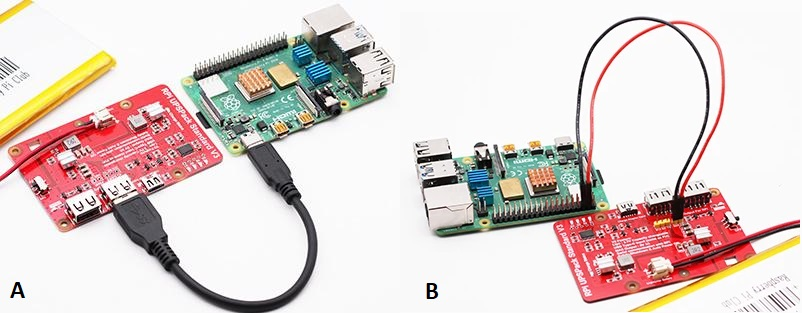
\includegraphics[width=0.5\textwidth]{connection.png}
	\caption{The Raspberry Pi and power board connection.}
	\label{fig:connection}
\end{figure}  

Since all the components are available as shown 
in \cref{fig:components}, we could assemble 
all the parts in one piece and started testing the whole system.
We have used the zip tie to hold the components and to
make sure everything sticks together. After trying to use the 
nylon straps tape to attach the components to the drone,
we have figured out that it blocks the fan 
and sensors at the bottom of the drone, 
. As shown in 
\cref{fig:full-hardware}, all the parts are in one system. 
The test flight was smooth, and everything worked perfectly. 

\begin{figure}[p]
	\centering
	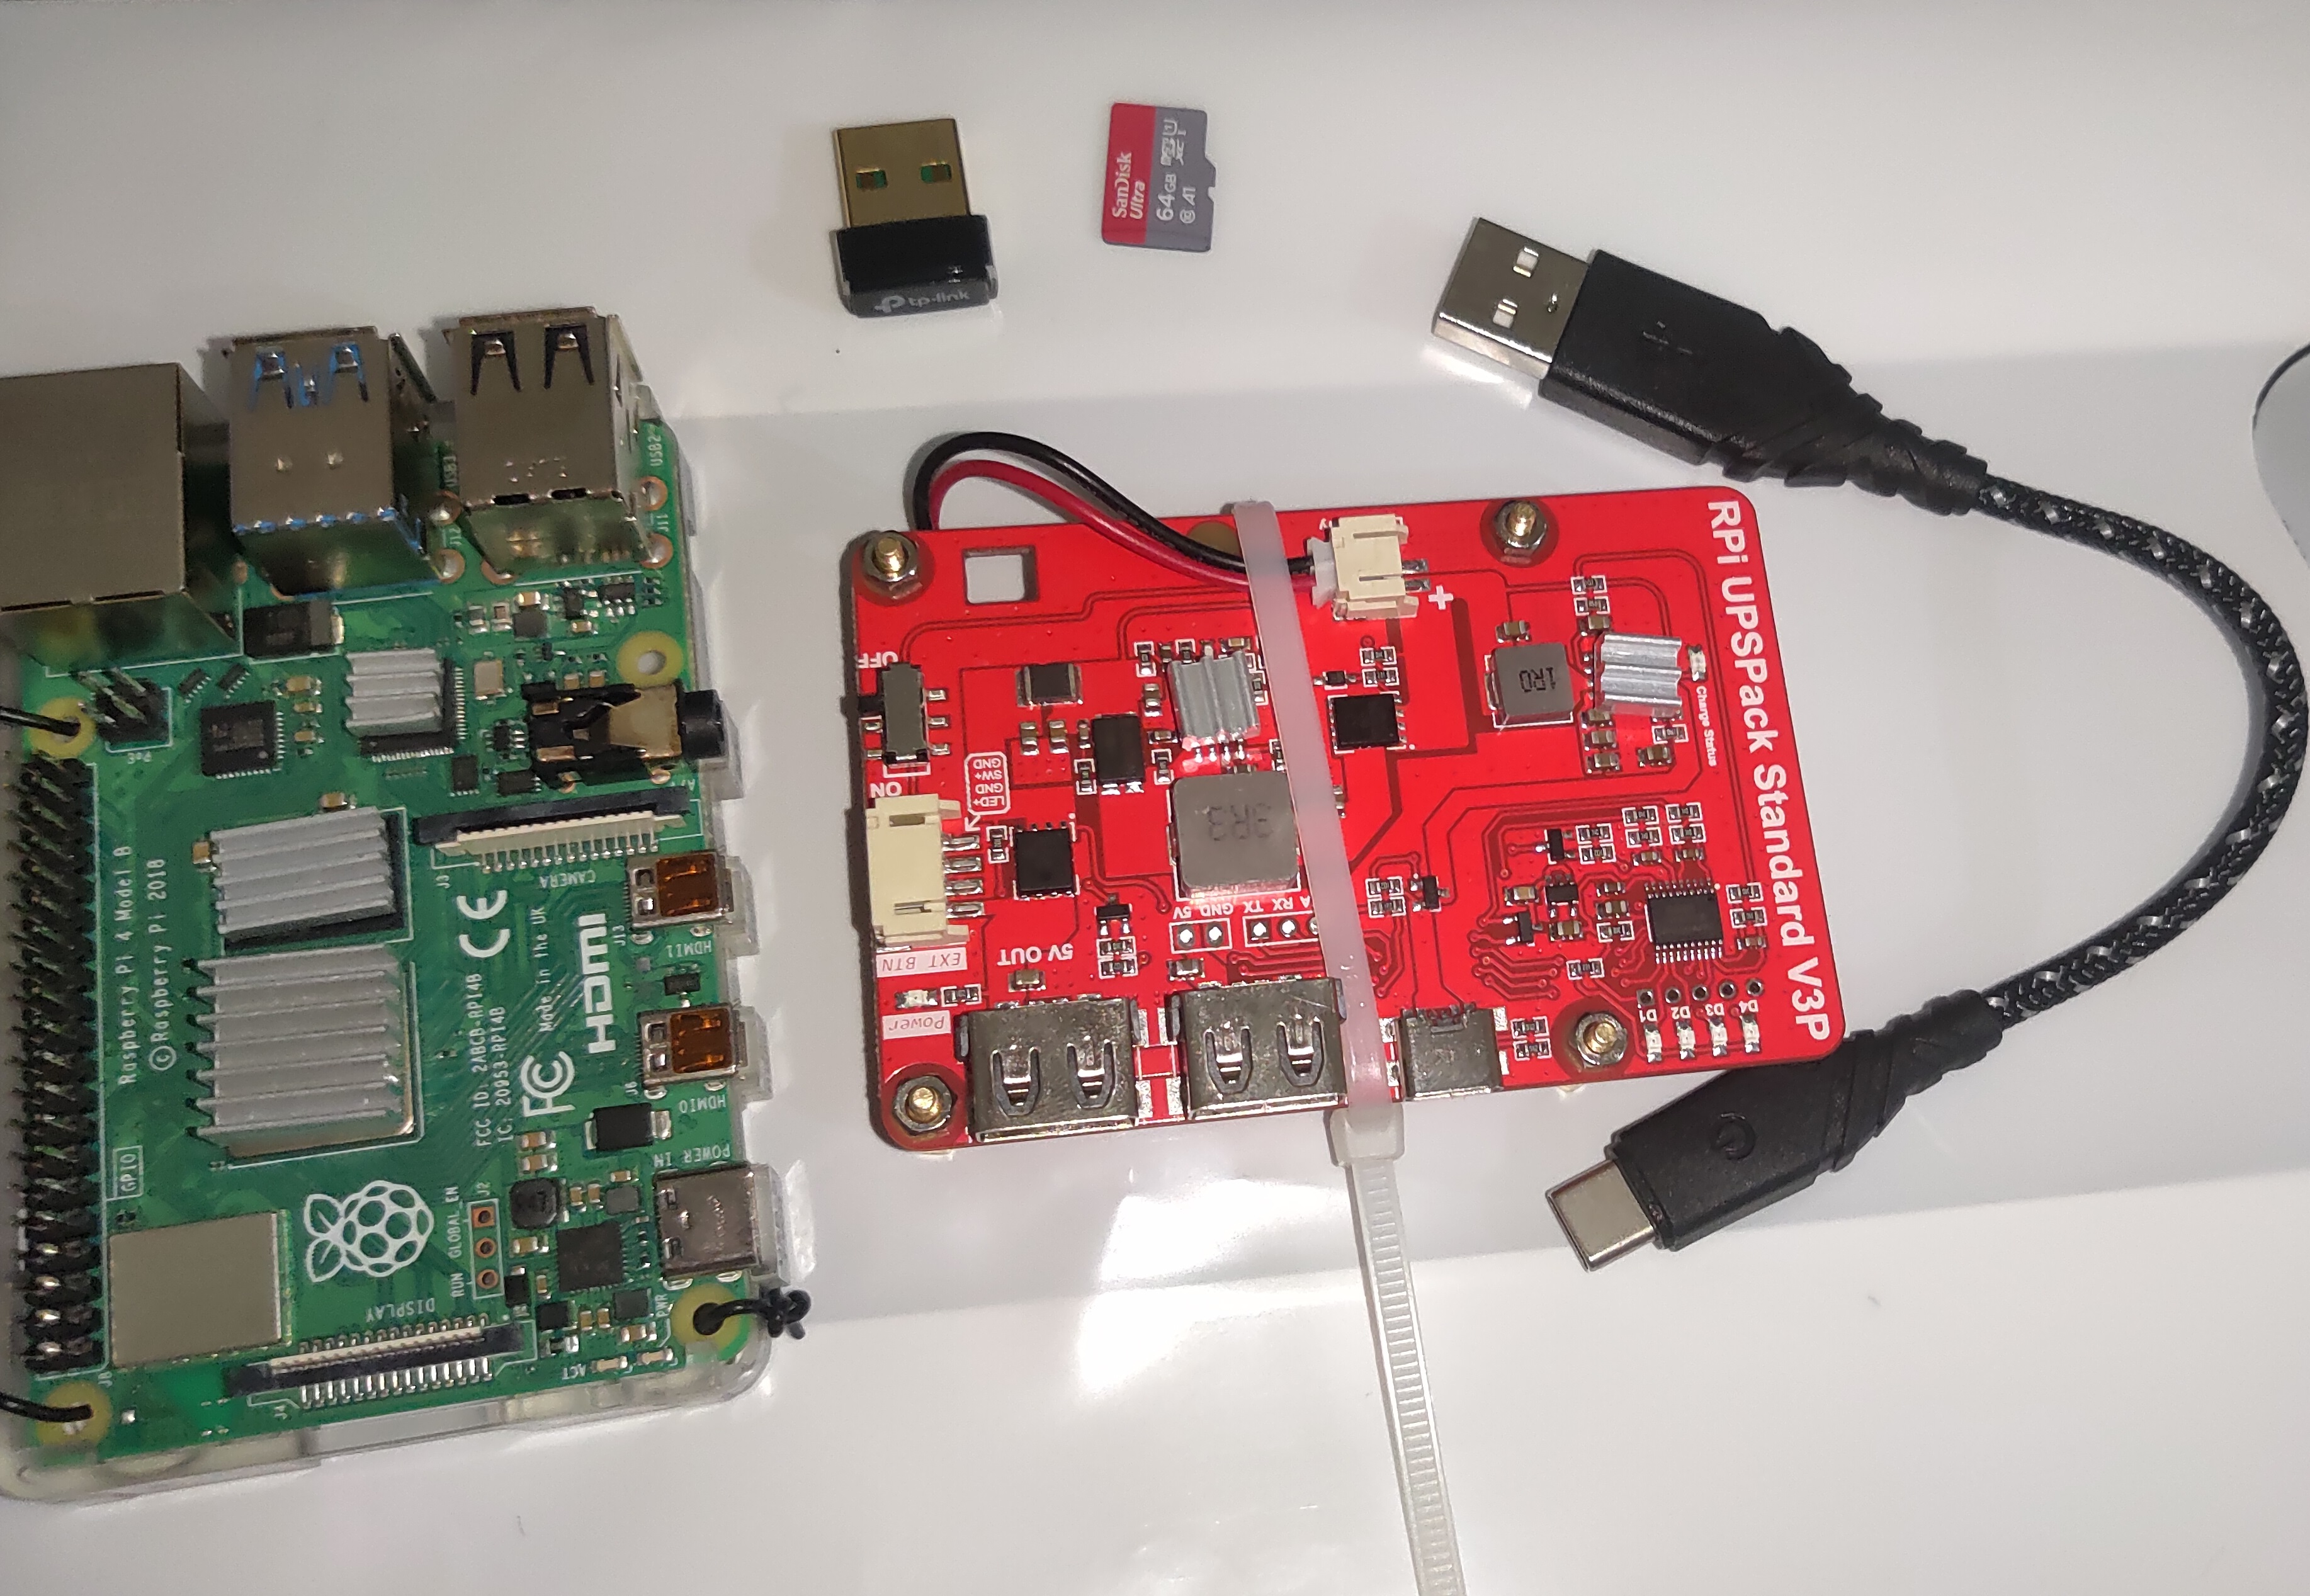
\includegraphics[width=0.5\textwidth]{components.jpg}
	\caption{All components needed.}
	\label{fig:components}
\end{figure}

\begin{figure}[p]
	\centering
	\includegraphics[width=0.6\textwidth]{full-drone-hardware.png}
	\caption{Full hardware system.}
	\label{fig:full-hardware}
\end{figure}  



\subsection{Reinforcement learning}

\lipsum[1]

\subsection{User interface}

\lipsum[1]

\end{document}
